\chapter{FUNCIONES DE VARIAS VARIABLES}
%\startcontents
\printchaptertableofcontents

El estudio de las funciones de varias variables constituye un pilar fundamental en el ámbito del Cálculo III, donde se exploran fenómenos matemáticos que implican más de una dimensión. A diferencia del cálculo de una sola variable, donde las funciones dependen únicamente de un parámetro, en el cálculo de varias variables, las funciones pueden depender de dos o más variables independientes. Este capítulo se adentra en la comprensión y análisis de estas funciones, explorando su comportamiento, propiedades y aplicaciones en diversos contextos.

En esencia, una función de varias variables asigna a cada punto en un dominio de dos o más dimensiones un único valor en el espacio real. Este enfoque multifacético permite modelar y comprender una amplia gama de fenómenos físicos, económicos y científicos, desde la trayectoria de un proyectil en el espacio hasta la distribución de temperatura en un sólido tridimensional.

La comprensión de las funciones de varias variables requiere el dominio de conceptos clave, entre ellos, la noción de dominio y rango, continuidad, derivadas parciales, gradientes, y optimización. A través del análisis de estas herramientas matemáticas, los estudiantes desarrollarán una perspicacia profunda sobre cómo las funciones de varias variables se comportan y cómo pueden ser utilizadas para resolver problemas prácticos.

Este capítulo se estructura para guiar al lector desde los conceptos básicos hasta las aplicaciones avanzadas. Comienza con la definición formal de una función de varias variables, examinando su representación gráfica y sus propiedades fundamentales. A medida que avanzamos, exploramos la diferenciabilidad y la integrabilidad de estas funciones, así como las técnicas para encontrar máximos y mínimos locales y absolutos.

%Además, se abordan aplicaciones relevantes en campos como la física, la ingeniería, la economía y las ciencias computacionales, ilustrando cómo las funciones de varias variables se utilizan para modelar situaciones del mundo real y resolver problemas complejos.

\section{Funciones y su dominio}

\begin{definition}
    Una función $f$ de dos variables es una regla que asigna a cada par ordenado de números reales $(x, y)$ de un conjunto $D$, un único número real que se denota con $f(x, y)$. El conjunto $D$ es el dominio de $f$ y su rango es el conjunto de valores que toma $f$, es decir, $\left\{ f(x, y) \mid (x, y) \in D \right\}$.
\end{definition}

A menudo, escribimos $z = f(x, y)$ para hacer explícito el valor que toma $f$ en el punto $(x, y)$. Las variables $x$ y $y$ son variables independientes y $z$ es la variable dependiente [compare lo anterior con la notación $y = f(x)$ para funciones de una variable].
\sideFigure[\label{fig:Funcion_dos_variables}]{
    \centering
    \includegraphics[width=\linewidth]{Images/Capitulo1/Funcion_dos_variables.pdf}
}

Una función de dos variables es una función cuyo dominio es un subconjunto de $\mathbb{R}^2$ y cuyo rango es un subconjunto de $\mathbb{R}$. Una manera de representar tal función es mediante un diagrama de flechas (véase la figura \ref{fig:Funcion_dos_variables}), donde el dominio $D$ se representa como un subconjunto del plano $x y$ y el rango es un conjunto de números sobre una recta real, que se muestra como un eje $z$. %Por ejemplo, si $f(x, y)$ representa la temperatura en un punto $(x, y)$ en una placa metálica plana con la forma de $D$, podemos considerar al eje $z$ como un termómetro que va mostrando el registro de temperaturas.

Si una función $f$ está dada por una fórmula y no se especifica dominio alguno, entonces se entiende que el dominio de $f$ será el conjunto de parejas $(x, y)$ para el cual la expresión dada es un número bien definido.

\begin{example}
    Para las siguientes funciones, evalúe $f(3, 2)$ y determine y grafique el dominio.
    \begin{tasks}(2)
        \task $\displaystyle f(x, y) = \frac{\sqrt{x + y + 1}}{x - 1}$
        \task $f(x, y) = x \ln (y^2 - x)$
    \end{tasks}
    \solucion
    \begin{enumerate}[label=\alph*)]
        \item Tenemos que\sideFigure[\label{Fig:Dominio_1}Representación geométrica del dominio de $\displaystyle f(x, y) = \frac{\sqrt{x + y + 1}}{x - 1}$]{
        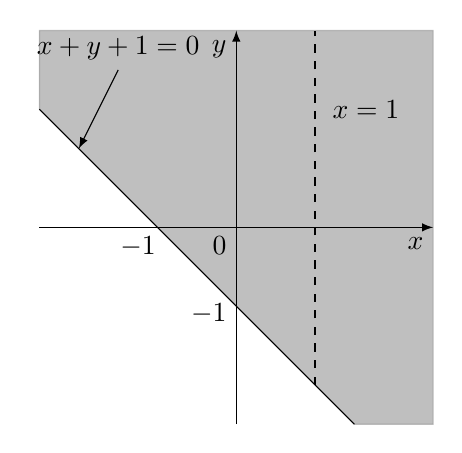
\begin{tikzpicture}
            \filldraw[gray,opacity=0.5] (1.5,-2.5) --(2.5,-2.5) -- (2.5,2.5) -- (-2.5,2.5) -- (-2.5,1.5) -- (1.5,-2.5) -- cycle;
            \draw[-latex] (-2.5,0) -- (2.5,0) node[below left] {$x$};
            \draw[-latex] (0,-2.5) -- (0,2.5) node[below left] {$y$};
            \draw (-2.5,1.5) -- (1.5,-2.5);
            \draw[latex-] (-2,1) -- (-1.5,2) node[above] {$x + y + 1 = 0$};
            \node[below left] at (0,0) {$0$};
            \node[below left] at (-0.9,0) {$-1$};
            \node[left] at (0,-1.1) {$-1$};
            \draw[dash pattern=on 3pt off 3pt] (1,-2) -- (1,2.5);
            \node[right] at (1.1,1.5) {$x = 1$};
        \end{tikzpicture}
        }
        $$f(3, 2) = \frac{\sqrt{3 + 2 + 1}}{3 - 1} = \frac{\sqrt{6}}{2}$$
        La expresión para $f$ tiene sentido si el denominador no es cero y la cantidad dentro del signo de raíz cuadrada es no negativa. Entonces, el dominio de $f$ es
        $$D = \left\{ (x, y) \in \RR[2] \mid x + y + 1 \geq 0, x \neq 1 \right\}.$$
        La desigualdad $x + y + 1 \geq 0$, o bien, $y \geq -x - 1$, describe los puntos que quedan en o por arriba de la recta $y = -x - 1$, mientras que $x \neq 1$ significa que los puntos sobre la recta $x = 1$ tienen que ser excluidos del dominio. Vea la figura \ref{Fig:Dominio_1}.
        \item Tenemos que\sideFigure[\label{Fig:Dominio_2}Representación geométrica del dominio de $f(x, y) = x \ln (y^2 - x)$]{
        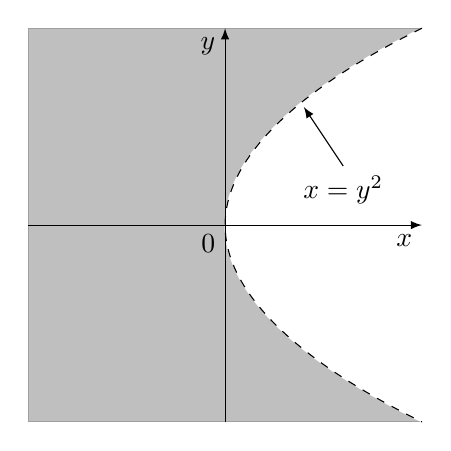
\begin{tikzpicture}
            \filldraw[gray,opacity=0.5] (-2.5,-2.5) rectangle (2.49,2.5);
            \node[below left] at (0,0) {$0$};
            \filldraw[rotate=-90,white] (-2.5,2.5) parabola bend (0,0) (2.5,2.5);
            \draw[rotate=-90,dash pattern=on 3pt off 3pt] (-2.5,2.5) parabola bend (0,0) (2.5,2.5);
            \draw[latex-] (1,1.5) -- (1.5,0.75) node[below] {$x = y^2$};
            \draw[-latex] (-2.5,0) -- (2.5,0) node[below left] {$x$};
            \draw[-latex] (0,-2.5) -- (0,2.5) node[below left] {$y$};
        \end{tikzpicture}
        }
        $$f(3, 2) = 3 \ln (2^2 - 3) = 0.$$
        Puesto que $\ln(y^2 - x)$ se define solo cuando $y^2 - x > 0$, es decir, $x < y^2$, el dominio de $f$ es
        $$D = \left\{ (x, y) \in \RR[2] \mid x < y^2 \right\}.$$
        Este es el conjunto de puntos a la izquierda de la parábola $x = y^2$. Vea la figura \ref{Fig:Dominio_2}.
    \end{enumerate}
\end{example}

\begin{example}
    Determine y grafique el dominio de las siguientes funciones:
    \begin{tasks}(2)
        \task $f(x, y) = \sqrt{x^2 + y^2 - 1}$
        \task $f(x, y) = \ln (x^2 + y^2 - 1)$
    \end{tasks}
    \newpage
    \solucion \sideFigure[\label{Fig:Dominio_3}Representación geométrica del dominio de $f(x, y) = \sqrt{x^2 + y^2 - 1}$]{
    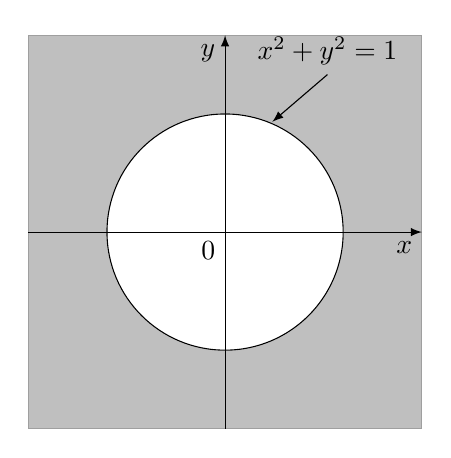
\begin{tikzpicture}
        \filldraw[gray,opacity=0.5] (-2.5,-2.5) rectangle (2.5,2.5);
        \filldraw[white] (0,0) circle (1.5cm);
        \draw (0,0) circle (1.5cm);
        \draw[-latex] (-2.5,0) -- (2.5,0) node[below left] {$x$};
        \draw[-latex] (0,-2.5) -- (0,2.5) node[below left] {$y$};
        \node[below left] at (0,0) {$0$};
        \draw[latex-] (0.6,1.4) -- (1.3,2) node[above] {$x^2 + y^2 = 1$};
    \end{tikzpicture}
    }
    \begin{enumerate}[label=\alph*)]
        \item Siguiendo la misma idea el ejemplo anterior, la expresión para $f$ tiene sentido si la cantidad dentro del signo de raíz cuadrada es no negativa. Así, el dominio de $f$ es
        $$D = \left\{ (x, y) \in \RR[2] \mid x^2 + y^2 - 1 \geq 0 \right\}.$$
        La desigualdad $x^2 + y^2 - 1 \geq 0$, o bien, $x^2 + y^2 \geq 1$, describe los puntos que quedan en o fuera de la circunferencia $x^2 + y^2 = 1$.
        \item Puesto que $\ln (x^2 + y^2 - 1)$ se define solo cuando $x^2 + y^2 - 1 > 0$, es decir, $x^2 + y^2 > 1$ el dominio de $f$ es\sideFigure[\label{Fig:Dominio_4}Representación geométrica del dominio de $f(x, y) = \ln (x^2 + y^2 - 1)$]{
        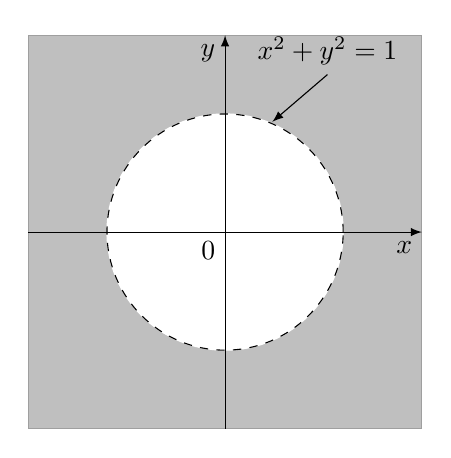
\begin{tikzpicture}
            \filldraw[gray,opacity=0.5] (-2.5,-2.5) rectangle (2.5,2.5);
            \filldraw[white] (0,0) circle (1.5cm);
            \draw[dash pattern=on 3pt off 3pt] (0,0) circle (1.5cm);
            \draw[-latex] (-2.5,0) -- (2.5,0) node[below left] {$x$};
            \draw[-latex] (0,-2.5) -- (0,2.5) node[below left] {$y$};
            \node[below left] at (0,0) {$0$};
            \draw[latex-] (0.6,1.4) -- (1.3,2) node[above] {$x^2 + y^2 = 1$};
        \end{tikzpicture}
        }
        $$D = \left\{ (x, y) \in \RR[2] \mid x^2 + y^2 > 1 \right\}.$$
        Este es el conjunto de puntos que están fuera de la circunferencia sin tomar los puntos que están en $x^2 + y^2 = 1$.
    \end{enumerate}
\end{example}

\section{Gráficas de funciones y curvas de nivel}

\begin{reminder}
    Es importante destacar que el círculo es un caso particular de la elipse, pues recordemos que la expresión para una circunferencia centrada en el origen está dada por
    $$x^2 + y^2 = r^2$$
    donde $r$ es el radio de dicha circunferencia y es una constante real, mientras que una elipse está dada por
    $$\frac{x^2}{a^2} + \frac{y^2}{b^2} = 1$$
    siendo $a$ y $b$ constantes reales. Generalmente la elipse tiene dos ejes de diferentes longitudes y dos focos distintos, pero el círculo es una forma particular de elipse donde ambos ejes son idénticos y los dos focos coinciden en el centro del círculo. La elipse puede presentarse de dos maneras distintas: horizontalmente o verticalmente. Cuando decimos que una elipse está en posición horizontal, significa que su eje mayor se extiende más en el eje $x$, mientras que en la posición vertical, el eje mayor se extiende más en el eje $y$.
    \begin{figure}[h!]
        \centering
        \subfloat[Elipse horizontal: Cuando $a>b$]{
        \begin{tikzpicture}[scale=0.9]
            \draw[-latex] (-3,0) -- (3,0) node[below left] {$x$};
            \draw[-latex] (0,-3) -- (0,3) node[below left] {$y$};
            \draw (0,0) ellipse (2cm and 1cm);
        \end{tikzpicture}
        } \hfill
        \subfloat[Elipse vertical: Cuando $b>a$]{
        \begin{tikzpicture}[scale=0.9]
            \draw[-latex] (-3,0) -- (3,0) node[below left] {$x$};
            \draw[-latex] (0,-3) -- (0,3) node[below left] {$y$};
            \draw (0,0) ellipse (1cm and 2cm);
        \end{tikzpicture}
        }
        \caption{Representación de la elipse}
    \end{figure}
    
    \noindent La hipérbole es otra cónica, al igual que la elipse. Sin embargo, a diferencia de la elipse que tiene una forma cerrada, la hipérbole es una curva abierta que se extiende hacia el infinito en ambas direcciones. En términos algebraicos, la ecuación de una hipérbole con centro en el origen se expresa como:
    $$\frac{x^2}{a^2} - \frac{y^2}{b^2} = 1$$
    donde $a$ y $b$ son constantes reales. Al igual que la elipse, la hipérbole puede presentarse en dos configuraciones principales: horizontal y vertical. En el caso de una hipérbole horizontal, las ramas principales de la hipérbole se extienden horizontalmente a lo largo del eje $x$, mientras que en una hipérbole vertical, las ramas principales se extienden verticalmente a lo largo del eje $y$.
    \begin{figure}[h!]
        \centering
        \subfloat[Hipérbole horizontal: Cuando $a>b$]{
        \begin{tikzpicture}[scale=0.9]
            \draw[-latex] (-3,0) -- (3,0) node[below left] {$x$};
            \draw[-latex] (0,-3) -- (0,3) node[below left] {$y$};
            \draw[rotate=90,yshift=1cm] (-2,2) parabola bend (0,0) (2,2);
            \draw[rotate=-90,yshift=1cm] (-2,2) parabola bend (0,0) (2,2);
        \end{tikzpicture}
        } \hfill
        \subfloat[Hipérbole vertical: Cuando $b>a$]{
        \begin{tikzpicture}[scale=0.9]
            \draw[-latex] (-3,0) -- (3,0) node[below left] {$x$};
            \draw[-latex] (0,-3) -- (0,3) node[below left] {$y$};
            \draw[yshift=1cm] (-2,2) parabola bend (0,0) (2,2);
            \draw[rotate=180,yshift=1cm] (-2,2) parabola bend (0,0) (2,2);
        \end{tikzpicture}
        }
        \caption{Representación de la hipérbole}
    \end{figure}
\end{reminder}\sideFigure[]{
\tdplotsetmaincoords{75}{110}
\begin{tikzpicture}[tdplot_main_coords,scale=2]
    \draw[thick,-latex] (0,0,0) coordinate(O) -- (2.5,0,0) node[anchor=north east] (x) {$x$};
    \draw[thick,-latex] (0,0,0) -- (0,1.5,0) node[anchor=north west] (y) {$y$};
    \draw[thick,-latex] (0,0,0) -- (0,0,2.5) node[anchor=south] (z) {$z$};
    \begin{scope}[xshift=0mm,rotate=-10]
        \tikzfading[name=fade right,
            left color=transparent!00,
            right color=transparent!60] ;
            \filldraw[black!30,path fading=fade right,fill opacity=0.5,
            ]  plot[variable=\x,samples=180,domain=-90:270] ({1.2*cos(\x)},{sin(\x)},{0});
            \draw plot[variable=\x,samples=180,domain=-90:270] ({1.2*cos(\x)},{sin(\x)},{0});
    \end{scope}
    \coordinate[label={[name=Plabel,xshift=0.5cm,yshift=1.7cm]above right:{$\big(x, y, f(x, y)\big)$}}] (P) at (0.2,0.5,1.2);
    \draw[-latex,shorten >=2.5pt] (Plabel) --(P);
    \fill (P) circle (1pt);
    \coordinate[label=below:{$(x, y, 0)$}] (Q) at (0.2,0.5,0);
    \fill (Q) circle (1pt);
    \draw[thick,] (P) -- (Q);
    \draw[thick,decoration={brace,raise=2.5pt},decorate] (P) -- (Q) node[midway,right=2mm]{$f(x, y)$};
    \draw[fill=gray,fill opacity=0.5,name path=back,->] plot[variable=\x,samples=180,domain=50:270] ({1.2*cos(\x)},{sin(\x)},{1.2+0.4*cos(2*\x)}) to[out=30,in=160] cycle;
    \draw[fill=gray,fill opacity=0.5,name path=front] plot[variable=\x,samples=180,domain=-90:50] ({1.2*cos(\x)},{sin(\x)},{1.2+0.4*cos(2*\x)}) to[out=160,in=30] cycle;
\end{tikzpicture}
}
\sideFigure[Un ejemplo común de las curvas de nivel son los mapas topográficos de regiones montañosas]{
\includegraphics[width=\linewidth]{Images/Capitulo1/Cartografico.pdf}
}
Otro modo de visualizar el comportamiento de una función de dos variables es considerar su gráfica

\begin{definition}
    Si $f$ es una función de dos variables con dominio $D$, entonces la gráfica de $f$ es el conjunto de todos los puntos $(x, y, z)$ en $\RR[3]$ tal que $(x, y)$ y $z = f(x, y)$ está en $D$.
\end{definition}

Un método para poder graficar funciones de dos funciones es mediante un mapa de curvas de nivel en el cual puntos de elevación igual se unen para formar líneas de contorno o curvas de nivel. Las curvas de nivel son líneas imaginarias que se utilizan para representar superficies tridimensionales en dos dimensiones, como mapas topográficos o gráficos de funciones de dos variables. Estas curvas conectan puntos que tienen la misma altura o el mismo valor de la función en el caso de las superficies. Por ejemplo, en un mapa topográfico, las curvas de nivel unen puntos que tienen la misma elevación sobre el nivel del mar. Al observar estas curvas, podemos entender la variación de la elevación o la función en diferentes áreas de la superficie, lo que proporciona una representación visual y comprensible del terreno o de la función en cuestión. Las curvas de nivel son una herramienta poderosa en diversas áreas, desde la cartografía hasta la ingeniería y las ciencias ambientales, facilitando la interpretación y el análisis de datos espaciales y funcionales.

\begin{definition}
    Las \textbf{curvas de nivel} de una función $f$ de dos variables son las curvas cuyas ecuaciones son $f(x, y) = k$, donde $k$ es una constante real.
\end{definition}